\section{Grundlagen} \label{grundlagenKapitel}
\acresetall
\subsection{Aufbau des \acl{ebuef}s}
Das \ac{ebuef} ist unterteilt in ein eingleisiges nicht-elektrifiziertes und ein zweigleisiges elektrifiziertes Streckennetz, welche über die Betriebsstelle Leopoldsgrün miteinander verbunden sind. In der Abbildung \ref{fig:ebuefNetz} ist das eingleisige Netz in schwarz dargestellt und die zweigleisige Hauptstrecke in rot.
\begin{figure}
  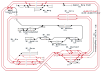
\includegraphics[width=\linewidth]{../images/netz/plan.pdf}
  \caption[Schienennetz des \ac{ebuef}s]{Schienennetz des \ac{ebuef}s (Quelle: www.ebuef.de/das-betriebsfeld/stellwerke; Letzter Zugriff am: 4. September 2021)}
  \label{fig:ebuefNetz}
\end{figure}
Das eingleisige Netz ist in \acp{infra} - welche mit Blockstrecken vergleichbar sind und eine Zugfolge im festen Raumabstand ermöglichen - eingeteilt.\footnote{\citet[S. 7, 42]{pachl1999systemtechnik}} Die \acp{infra} sind mit der RailCom-Technik ausgestattet, welche über die Decoder in den Fahrzeugen den aktuellen \ac{infra} ermittelt und diesen in der \textit{fma}-Tabelle der \textit{MySQL}-Datenbank speichert.\footnote{\cite{railcomnorm}} Zudem sind in der Datenbank alle Informationen über die Infrastruktur gespeichert. Für die Fahrzeugsteuerung essentiell sind dabei die aktuellen Signalbegriffe aller Signale und die Längen der \acp{infra}.\footnote{\cite{ebuef}}

Für den Betrieb des \ac{ebuef}s muss eine neue Session angelegt werden und gestartet werden. Der Start der Session muss vor dem Start der Fahrzeugsteuerung erfolgen, da die Fahrzeugsteuerung beim Start alle benötigten Informationen der Session einliest.
\subsection{Aufbau der \textit{MySQL}-Datenbank}
Alle Informationen und Daten, die für den Betrieb des \ac{ebuef}s benötigt werden, werden in einer \textit{MySQL}-Datenbank gespeichert. In der Tabelle \ref{table:sqldatenbank} werden die wichtigsten Tabellen der Datenbank aufgelistet und kurz beschrieben.
\begin{table}
\begin{center}
\renewcommand{\arraystretch}{1.2}
\begin{tabular}{c|c}
Name & Beschreibung \\ \hline
\textit{fahrplan\_sessionfahrplan}   	&   	Fahrpläne der Session für alle Fahrzeuge                  \\ \hline
\textit{fahrzeuge}                 		&   	Fahrzeuge                  \\ \hline
\textit{fahrzeuge\_baureihen}&   	Baureiheninformationen                  \\ \hline
\textit{fahrzeuge\_daten}      &   	Statische Daten der Fahrzeuge                  \\ \hline
\textit{fma}                 		&   	Freimeldeabschnitte                  \\ \hline
\textit{gbt\_fma}                 		&   	\makecell{Zuordnung der GBT-Abschnitte,\\FMA-Abschnitte und \acp{infra}}                   \\ \hline
\textit{infra\_daten}           &   	Statische Daten der Infrastruktur                  \\ \hline
\textit{infra\_zustand}       &   	Zustand der Infrastruktur                  \\ \hline
\textit{signale}                 		&   	Standorte der Signale                  \\
\end{tabular}
\renewcommand{\arraystretch}{1}
\caption{Beschreibung der wichtigsten Tabellen der \textit{MySQL}-Datenbank}
\label{table:sqldatenbank}
\end{center}
\end{table}
\subsection{Ziele und Prioritätssetzung der Fahrzeugsteuerung}
An oberster Priorität der Fahrzeugsteuerung steht eine möglichst effiziente Umsetzung und das Einhalten der vorgegebenen Fahrpläne. Für eine effiziente Umsetzung wurden die Zugriffe auf die \textit{MySQL}-Datenbank während des laufenden Betriebs der Fahrzeugsteuerung möglichst minimal gehalten und Teile des Quellcodes, welche häufiger verwendet werden, in Funktionen ausgelagert. Die Ermittlung der \glspl{fahrtverlauf} berücksichtigt für die Einhaltung der Fahrplanzeiten neben den Ankunfts- und Abfahrtszeiten auch die aktuelle Verspätung und versucht diese auszugleichen.

An zweiter Stelle der Prioritätssetzung steht das energieeffiziente Fahren. Damit die Fahrten möglichst energieeffizient sind, fahren die Züge die kleinstmöglichste Geschwindigkeit, bei der das Ziel ohne eine Verspätung erreicht wird. Sollte auch bei der größtmöglichen Geschwindigkeit das Ziel mit einer Verspätung erreicht werden, wird diese Geschwindigkeit gewählt und die Verspätung so möglichst gering gehalten. In dem Fall, dass es für ein Fahrzeug möglich ist mit einer geringeren Geschwindigkeit zu fahren, als die maximal zulässige Geschwindigkeit, wird die Geschwindigkeit möglichst am Ende des \gls{fahrtverlauf}s reduziert. Dadurch hat das Fahrzeug, für den Fall einer Fahrstraßenänderung oder Reduzierung der zulässigen Höchstgeschwindigkeit, möglichst viel Zeitpuffer.
\newpage
\subsection{Fahrdynamik}
In der Realität gibt es vier Bewegungsphasen, in denen sich ein Fahrzeug befinden kann:
\begin{itemize}
\item Anfahren
\item Beharrungsfahrt
\item Auslauf
\item Bremsen
\end{itemize}
Beim Anfahren ist die Antriebskraft größer als die Summe der Widerstandskräfte, wodurch das Fahrzeug beschleunigt und in der Beharrungsfahrt entspricht die Antriebskraft der Summe der Widerstandskräfte, wodurch die Geschwindigkeit des Fahrzeugs konstant bleibt. Für die Reduzierung der Geschwindigkeit kann entweder die Antriebskraft gleich null sein oder eine Bremskraft aufgewendet werden.\footnote{\citet[S. 23 ff.]{pachl1999systemtechnik}}

Die Widerstandskräfte setzen sich aus dem Streckenwiderstand, dem Fahrzeugwiderstand und dem Anfahrwiderstand zusammen und lassen sich mit den gegebenen Daten nicht vollständig berechnen.\footnote{\citet[S. 25 ff.]{pachl1999systemtechnik}} Aus diesem Grund werden die Widerstandskräfte bei der Fahrzeugsteuerung nicht berücksichtigt und die Auslaufphase, welche nur von der Widerstandskräften abhängig ist, wird ebenfalls nicht berücksichtigt.
\subsection{Aufbau des Projekts}
In der Darstellung \ref{fig:aufbauProjekt} ist der Aufbau des gesamten Projekts und die für die Arbeit relevanten Dateien/Ordner dargestellt. Dateien, welche bereits vorhanden waren, sind die Funktionen mit einem Sternchen ($^\ast$) markiert. Die für die Fahrzeugsteuerung essentiellen Dateien befinden sich innerhalb des \textit{php}-Ordners, wobei die Datei \textit{main.php} die Fahrzeugsteuerung startet und für die Berechnung der Fahrtverläufe auf die Dateien in dem \textit{functions}-Unterordner zugreift. Die benötigten Dateien für den Zugriff auf die \textit{SQL}-Datenbank befinden sich in dem \textit{config}-Unterordner und global festgelegte Parameter sind in der Datei \textit{globalVariables.php} abgespeichert. Für die Visualisierung (siehe Kapitel \ref{visualisierungFahrtverlaeufe}) der Fahrtverläufe werden die Dateien aus dem \textit{matlab}- und \textit{json}-Ordner benötigt.
\begin{figure}
\begin{forest}
  dir tree
[project
[php
  	[main.php]
	[globalVariables.php]
	[db\_tables.php$^\ast$]
	[mysqli.php$^\ast$]
	[vorbelegung.php$^\ast$]
	[config
		[config.php$^\ast$]
		[db\_access.php$^\ast$]
		[multicast.php$^\ast$]
	]
	[functions
		[cache\_functions\_own.php]
		[ebuef\_functions.php$^\ast$]
		[fahrtverlauf\_functions.php]
		[sort\_functions.php]
	]	
  ]
  [matlab
  	[speedOverPosition.m]
	[\dots]
  ]
  [json
  	[\dots]
  ]
]
\end{forest}
\caption{Aufbau der Dateistrukturen}
\label{fig:aufbauProjekt}
\end{figure}